\documentclass[a4paper]{article}
\author {Vavilov Andrei}
\title {Animarea modelelor 3D folosind retele neuronale}

\usepackage[utf8]{inputenc}
\usepackage[T1]{fontenc}
\usepackage{textcomp}
\usepackage{amsmath, amssymb}
\usepackage[ht]{graphicx}
\usepackage{hyperref}
% figure support
\usepackage{import}
\usepackage{float}
\usepackage[backend=biber]{biblatex}
\addbibresource{bib.bib}
\usepackage{bookmark}

\pdfminorversion=7
\usepackage{pdfpages}
\usepackage{transparent}
\newcommand{\incfig}[1]{%
	\def\svgwidth{\columnwidth}
	\import{./figures/}{#1.pdf_tex}
}
\setlength{\parskip}{1em}
\pdfsuppresswarningpagegroup=1

\begin{document}

\maketitle

\section{Introducere}
    Inteligenta artificiala este un domeniu foarte versatil, a carui aplicabilitate poate fi extinsa in foarte multe
    domenii,printre care si modelarea grafica, mai exact in modelarea si animarea 3D.


    Urmatorul studiu isi propune sa prezinte o parte din modelele si tehnologiile care pot fi folosite pentru a
anima un model 3D in timp real, pe baza unui fisier audio selectat de catre utilizator.

\section{Tehnologii propuse}
Deoarece inteligenta artificiala este unul dintre cele mai intens cercetate domenii din prezent, exista o varietate de
tehnologii si instrumente pentru realizarea de proiecte.

In continuare voi prezenta si argumenta pe scurt alegerile facute.

\subsection{Limbajul de programare }
O intrebare care a aparut odata cu cresterea in populariate a domeniului inteligentei artificiale este
``Ce limbaj de programare ar trebui sa folosesc?''.Desi nu exista ``cel mai bun limbaj pentru inteligenta artificiala'', Python este de cele mai multe ori alegerea preferata atat a programatorilor cat si a oamenilor
de stiinta si a statisticienilor datorita:
\begin{enumerate}
	\item Varietatea de framework-uri si instrumente pentru Machine Learning, Data science si modelare/interpretare
		a datelor (TensorFlow, Scipy, Pytorch, Numpy, Pandas).
	\item Numarul mare de resurse disponibile online
	\item Sintaxa simpla
	\item Fiind un limbaj \textit{dinamically typed}, realizarea de aplicatii/modele este facila si rapida.
	\item Fiind un limbaj \textit{cross platform}, aplicatiile sunt automat suportate pe o varietate mare de
		platforme si sisteme de operare.
\end{enumerate}
\subsection{Tipul de \textit{Neural Network} folosit}
Inainte de a argumenta alegerea retelei neuronale, trebuie introdus pe scurt conceptul
de \textbf{\textit{Deep Learning}}.

\textit{Deep Learning}, cunoscut si sub numele de \textit{Deep Structured Learning},
face parte din familia invatarii automate si reprezinta o combinare a algoritmilor de \textit{Machine Learning} cu
\textit{Representation Learning} (tehnica de automatizare a interpretarii datelor). Principalul avantaj pe care
\textit{Deep Learning Neural Networks} il prezinta fata de algoritmii de \textit{Machine Learning} este minimizarea
interventiei factorului uman, prin automatizarea procesului de \textit{feauture extraction}, adica extragerea
caracteristicilor distinctive ale datelor de intrare.


Din categoria \textit{Deep Learning Neural
Networks} trebuie amintite \textbf{ANN, CNN, si RNN}, principalele categorii de \textit{Deep Learning Neural Networks}.
\begin{itemize}
	\label{NN}

	\item ANN

\begin{figure}[ht]
	\centering
	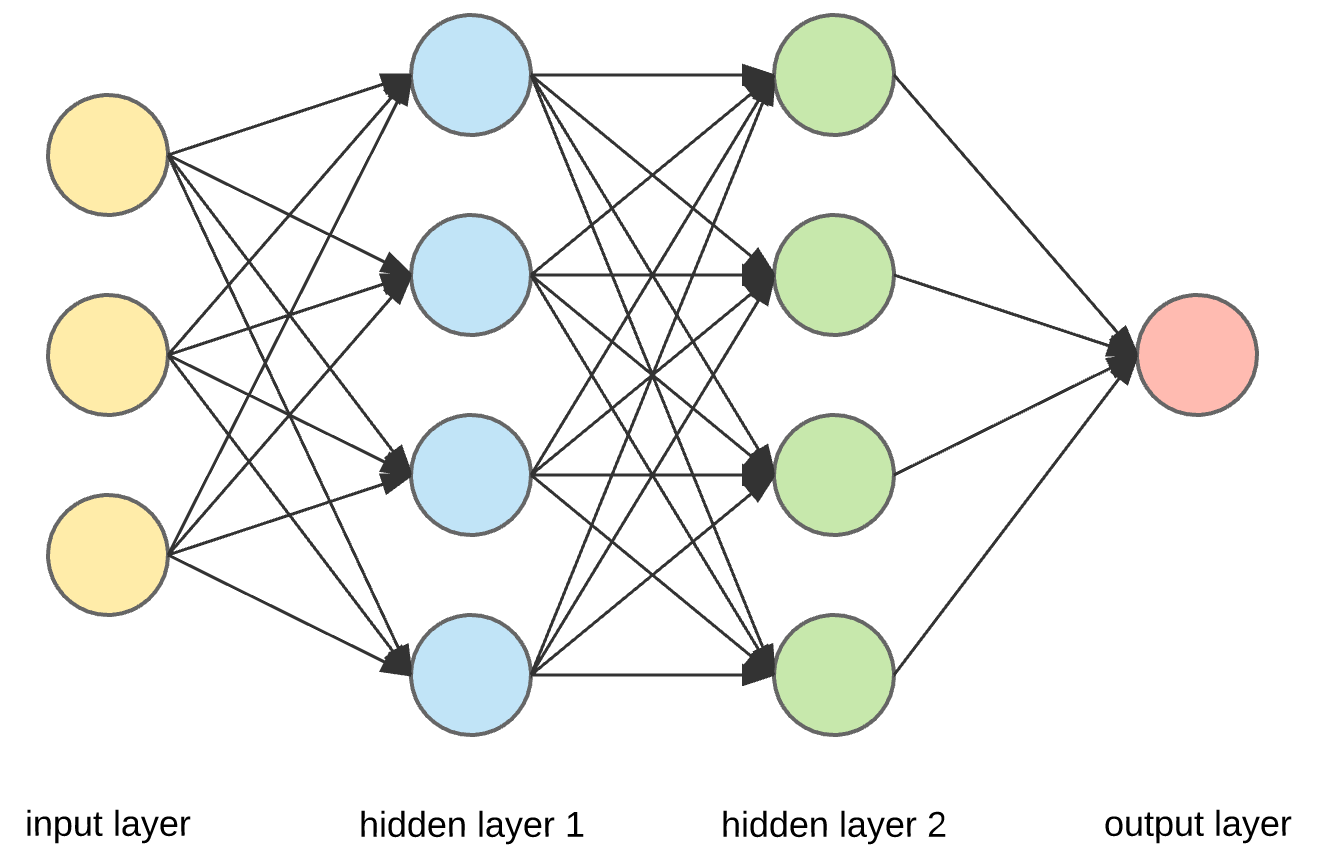
\includegraphics[width = 1.8in]{ann.png}
	\caption{Ilustrare schematica a arhitecturii ANN}
\label{ANN}
\end{figure}
Retelele neuronale de tip ANN au ca si caracteristica principala prelucrearea unidirectioanla a datelor (\textit{forward feeding})
si este un tip de retea preferata in general in cazul problemelor din spectrul buisness-ului( predictii in legatura cu vanzarile/
viitoarele interese ale cumparatorilor, validare de date, risk management, etc.).

	\item CNN
\begin{figure}[ht]
	\centering
	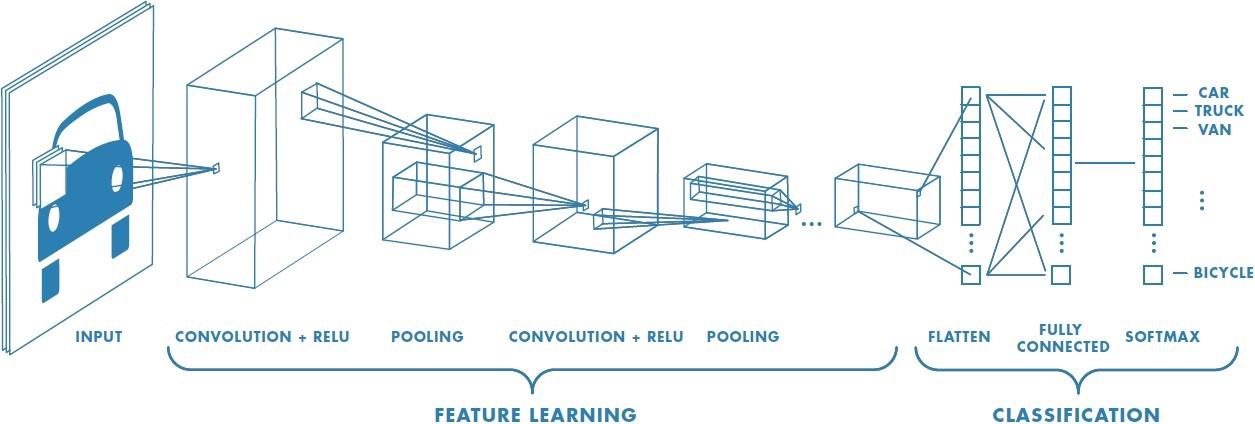
\includegraphics[width = 1.5in]{cnn.jpeg}
	\caption{Ilustrare schematica a arhitecturii CNN}
\label{CNN}
\end{figure}


Retelele neuronale de tip CNN sunt folosite in cadrul problemelor de clasificare a imaginilor, acestea prelucrand caracteristicile
spatiale(pozitia pixelilor si relatiile dintre acestia).

	\item RNN
\begin{figure}[ht]
	\centering
	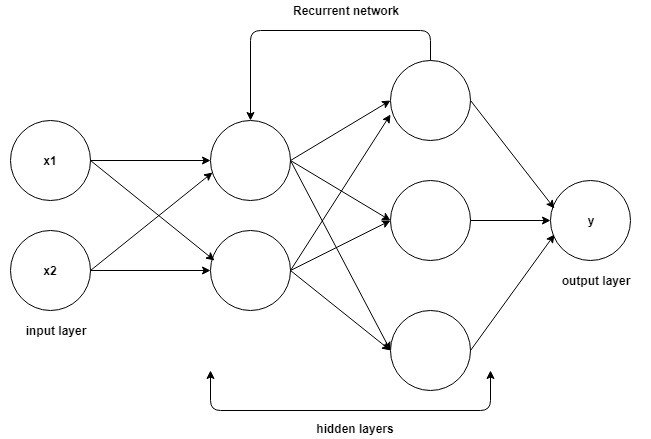
\includegraphics[width = 1.7in]{rnn.jpeg}
	\caption{Ilustrare schematica a arhitecturii RNN}
\label{RNN}

\end{figure}


Retelele neuronale de tip RNN, desi au o structura relativ asemanatoare cu ANN, se deosebesc prin capacitatea de a prelucra datele
in ambele directii (\textit{recurrent feeding}), fiind astfel o optiune valida preferata in cazul problemelor de procesare text
si audio. RNN transmite secvential informatia catre straturile de neuroni, determinand dependentele dintre componentele datelor
de intrare. Aceasta proprietate distinctiva se numeste \textit{Parameter sharing} si duce la scaderea numarului de neuroni necesari
din retea si, implicit, la scaderea costurilor computationale.

\end{itemize}


 \section {Aprofundarea tehnologiilor propuse }
 Clasificarea instrumentelor muzicale nu este o problema noua, aceasta fiind abordata de cercetatori in
invatare automata prin tehnici precum \textit{SVM} (rata de eroare de 30\% )
, si clasificare prin \textit{K-NN}.
In ultimii ani insa cercetarea s-a indreptat spre \hyperref[NN]{retele neuronale} deoarece acestea elimina nevoia unui factor uman
care sa extraga trasaturile datelor de intrare. Apare insa problema alegerii tipului de retea neuronala. Articolul \cite{DLFMIR}  compara arhitectura \textit{ leNet CNN } cu arhitectura \textit{LTSM} ( derivata din \textit{RNN}), acestea fiind
principalele candidate pentru rezolvarea problemei date.


Rezultatul experimentului a demonstrat ca, in urma antrenarii celor doua retele neuronale cu o multime de date
de intrare alcatuita din 200 de fisiere audio, cu lungime de aproximativ o secunda, arhitectura
\textit{leNet CNN} ajunge la o acuratete foarte apropiata de cea a \textit{LTSM} mult mai rapid, in timp ce
foloseste mult mai putine resurse, fiind deci o alegere mai buna pentru problema clasificarii de instrumente
muzicale. Urmatoarea figura ilustreaza rezulatele obtinute in urma testului dupa un antrenament de 100 de
epoci.

\begin{figure}[H]
	\centering
	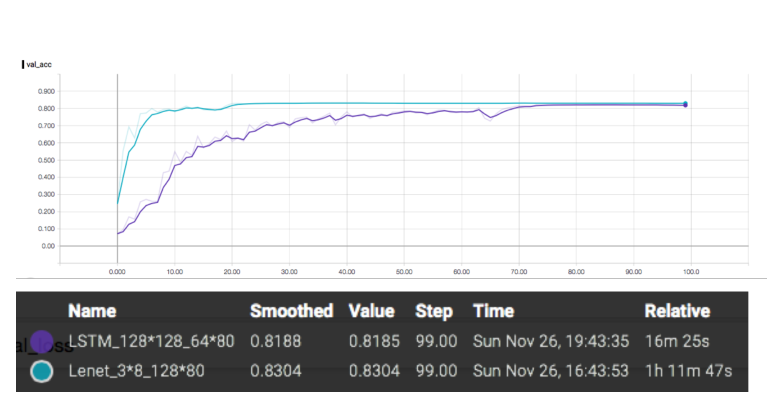
\includegraphics[width = 2.6in]{res.png}
	\caption{Rezultatele obtinute comparatiei dintre LSTM si leNet}
\label{result1}
\end{figure}


Pentru a transforma fisierele audio in input valid vom folosi spectograme \textit{Mel}. Pentru a intelege cum
functioneaza, este utila prezentarea conceptelor de \textit{semnale audio} si \textit{transformari Fourier}.


Un semnal reprezinta ilustrarea unui fenoment in timp. In cazul fisierelor audio, semnalele indica variatia
cantiatii de aer din timpul unei inregistrari. Aceasta variate este in general determinata prin masurarea la
intervale foarte mici ( 44.1kHz $\approx$ 44100 de inregistrari pe secunda).

\textit{Transformarea Fourier reprezinta} o tehnica de transformare matematica care descompune o functie
relativ la dependentele sale spatiale si temporale.
Semnalul audio este compus din unde sonore care ilustreaza doar amplitudinea unei anumite inregistrari.
\textit{Transforarea Fourier} permite convertirea de la o ilustrare temporala la o ilustrare a frecventei,
numita spectru.


\begin{figure}[H]
	\centering
	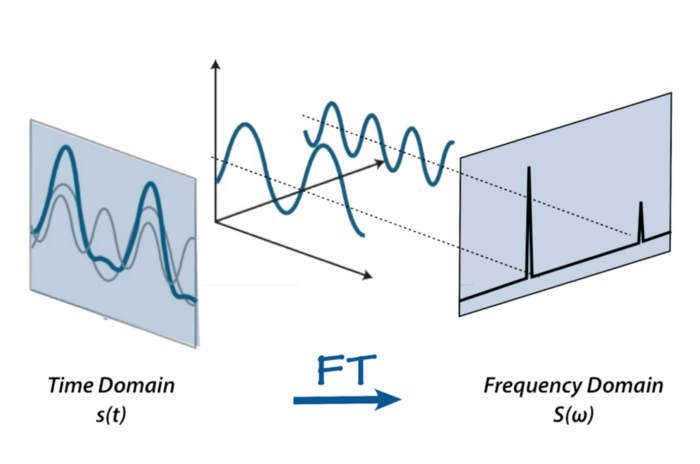
\includegraphics[width = 2.6in]{fourier.png}
	\caption{Procesul de tranformare Fourier}
\label{result2}
\end{figure}


O spectograma este o reprezentare grafica a aplicarii algoritmului de transformare Fourier peste semnale
nonperiodice. Spectogramele ilustreaza caracteristici ale sunetului precum nivelul de zgomot,amplitudinea,
variatia frecventei,nivelul de decibeli etc.



\begin{figure}[H]
	\centering
	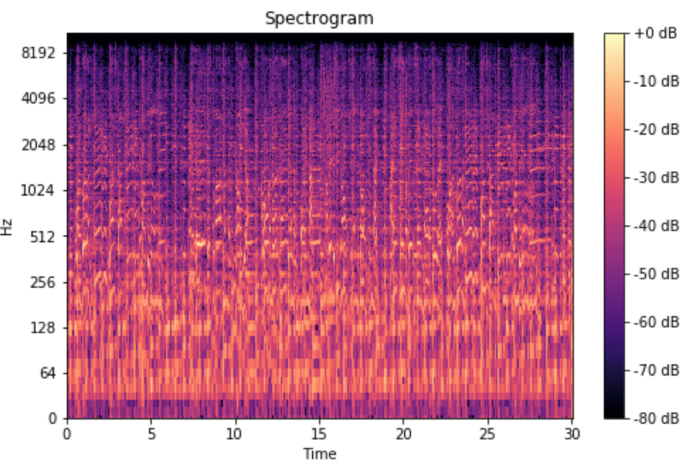
\includegraphics[width = 4.6in]{spec.png}
	\caption{Spectograma audio}
\label{result3}
\end{figure}


Scala \textit{Mel} este o reprezentare a sunetelor perceptibile de catre om. Aceasta este folosita pentru
normalizarea si eliminarea de caracteristici irelevante ale fisierelor audio.


Procesarea datelor de intrare pentru reteaua neuronala poate fi facilitata prin intermediul \textit{Spectogra
melor Mel}, transformand problema de recunoastere audio intr-o problema de recunastere a imaginilor.

\nocite{*}
\printbibliography[title=Bibliografie]
\end{document}
